% !TEX TS-program = pdflatex
% !TEX encoding = UTF-8 Unicode

% This is a simple template for a LaTeX document using the "article" class.
% See "book", "report", "letter" for other types of document.

\documentclass[11pt]{article} % use larger type; default would be 10pt

\usepackage[utf8]{inputenc} % set input encoding (not needed with XeLaTeX)

%%% Examples of Article customizations
% These packages are optional, depending whether you want the features they provide.
% See the LaTeX Companion or other references for full information.

%%% PAGE DIMENSIONS
\usepackage{geometry} % to change the page dimensions
\geometry{a4paper} % or letterpaper (US) or a5paper or....
% \geometry{margin=2in} % for example, change the margins to 2 inches all round
% \geometry{landscape} % set up the page for landscape
%   read geometry.pdf for detailed page layout information

\usepackage{graphicx} % support the \includegraphics command and options

% \usepackage[parfill]{parskip} % Activate to begin paragraphs with an empty line rather than an indent

%%% PACKAGES
\usepackage{booktabs} % for much better looking tables
\usepackage{array} % for better arrays (eg matrices) in maths
\usepackage{paralist} % very flexible & customisable lists (eg. enumerate/itemize, etc.)
\usepackage{verbatim} % adds environment for commenting out blocks of text & for better verbatim
\usepackage{subfig} % make it possible to include more than one captioned figure/table in a single float
% These packages are all incorporated in the memoir class to one degree or another...
\usepackage{amsmath}
\usepackage{amssymb}
%%% HEADERS & FOOTERS
\usepackage{fancyhdr} % This should be set AFTER setting up the page geometry
\pagestyle{fancy} % options: empty , plain , fancy
\renewcommand{\headrulewidth}{0pt} % customise the layout...
\lhead{}\chead{}\rhead{}
\lfoot{}\cfoot{\thepage}\rfoot{}

%%% SECTION TITLE APPEARANCE
\usepackage{sectsty}
\allsectionsfont{\sffamily\mdseries\upshape} % (See the fntguide.pdf for font help)
% (This matches ConTeXt defaults)

%%% ToC (table of contents) APPEARANCE
\usepackage[nottoc,notlof,notlot]{tocbibind} % Put the bibliography in the ToC
\usepackage[titles,subfigure]{tocloft} % Alter the style of the Table of Contents
\renewcommand{\cftsecfont}{\rmfamily\mdseries\upshape}
\renewcommand{\cftsecpagefont}{\rmfamily\mdseries\upshape} % No bold!

%%% END Article customizations

%%% The "real" document content comes below...

\title{Homework based on Chapter 5\\
Computational Probability and Statistics \\
CIS 2033, Section 002}
\author{}
\date{} % Activate to display a given date or no date (if empty),
         % otherwise the current date is printed 

\begin{document}
\maketitle

\section{Part 1 (Due: 9:00 AM, Friday, Feb. 13, 2015)}

\paragraph*{\bf Question 1} Let $X$ be a continuous random variable with probability density function\\
\begin{align*}
f(x) = \left\lbrace
\begin{array}{ll} 
\frac{7}{8} & \text{for } -\frac{1}{2} \leq x \leq \frac{1}{2} \\
& \\
\frac{1}{16} & \text{for } 3 \leq x \leq 5 \\ 
& \\
0 & \text{elsewhere.}
\end{array}
\right.
\end{align*}

\subparagraph*{a.} Draw the graph of $f$.
\subparagraph*{b.} Determine the distribution function of $F$ of $X$, and draw its graph. 


\paragraph*{\bf Question 2} The probability density function $f$ of a continuous random variable $X$ is given by: 
\begin{align*}
f(x) = \left\lbrace
\begin{array}{ll}
C(4x - 2x^2)  & \text{for } 0 \leq x \leq 2 \\
0 & \text{elsewhere.}
\end{array} \right.
\end{align*}

\subparagraph*{a.} Compute $c$. 
\subparagraph*{b.} Compute the distribution function $F$ of $X$.
\subparagraph*{c.} Compute $F(1)$ and $P(X>1)$
\vspace{8em}
\section{Part 2 (Due: 11:59 PM, Tuesday, Feb. 17, 2015)}
\paragraph*{\bf Question 3}Suppose we choose arbitrarily a point from the square with corners at $(2, 1), (3, 1), (2, 2), (3, 2)$. The random variable $A$ is the area of the triangle with its corners at $(2, 1), (3, 1)$ and the chosen point. 

\subparagraph*{a.} What is the largest area $A$ that can occur, and what is the set of points for which $A \leq \frac{1}{4}$ ?
\subparagraph*{b.} Determine the distribution function $F$ of $A$. 
\subparagraph*{c.} Determine the probability density function $f$ of $A$.
\paragraph*{\bf Question 4}
Compute the median of an $Exp(3)$ distribution. 
\paragraph*{\bf Question 5}
 Compute the median of a $Par(1)$ distribution. 
\newpage

\section*{\bf Appendix}
\paragraph*{5.1} Let $X$ be a continuous random variable with probability density function\\
\begin{align*}
f(x) = \left\lbrace
\begin{array}{ll} 
\frac{3}{4} & \text{for } 0 \leq x \leq 1 \\
& \\
\frac{1}{4} & \text{for } 2 \leq x \leq 3 \\ 
& \\
0 & \text{elsewhere.}
\end{array}
\right.
\end{align*}

\subparagraph*{a.} Draw the graph of $f$.
The Probability density function is in Figure~\ref{Fig:ch0501a}.
\begin{figure}[h!]
\centering
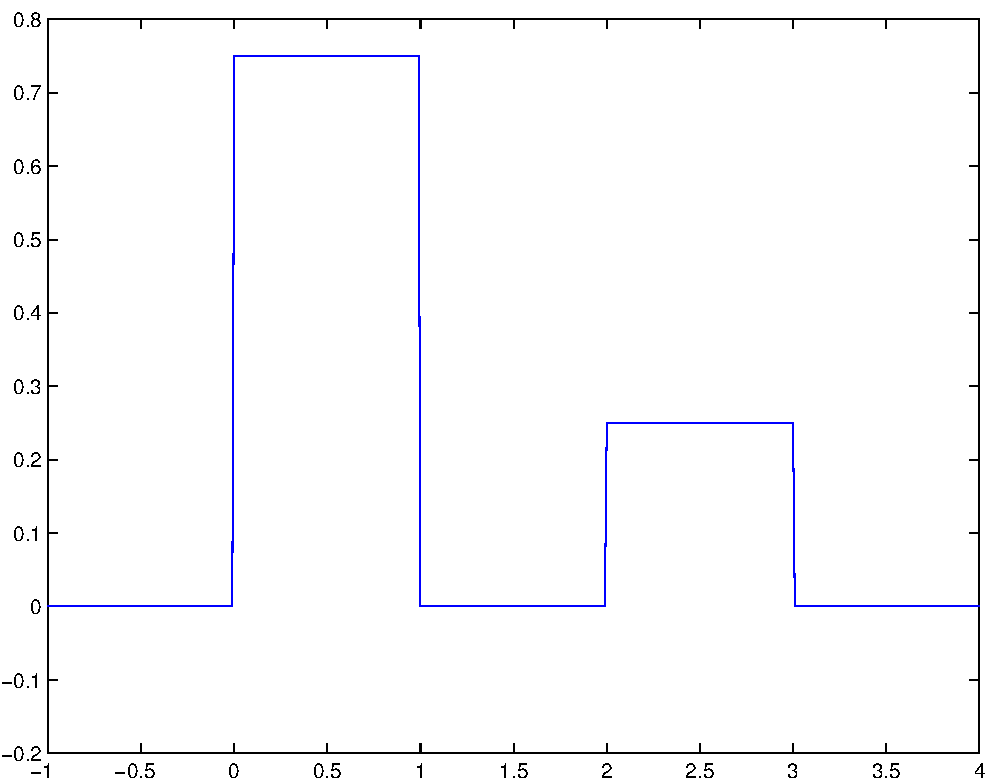
\includegraphics[width=3in, height=1.5in]{ch0501a}
\caption{Probability density function $f$.}
\label{Fig:ch0501a}
\end{figure}

\subparagraph*{b.} Determine the distribution function of $F$ of $X$, and draw its graph. 
We first show how to compute the distribution function, 
\begin{enumerate}
\item If $a < 0$, then 
\begin{align*}
F(a) = & \int_{-\infty}^a 0 dx  \\
& =  0 
\end{align*} 
\item If $0 \leq a < 1$, then 
\begin{align*}
F(a) = & \int_{-\infty}^0 0 dx + \int_{0}^a \frac{3}{4} dx \\
& = 0 + \left[\frac{3x}{4}\right]_{0}^a \\
& = \frac{3a}{4}
\end{align*}
\item If $1 \leq a < 2$, then
\begin{align*}
F(a) = & \int_{-\infty}^0 0 dx + \int_{0}^1 \frac{3}{4} dx + \int_{1}^a 0 dx \\
& = 0 + \left[\frac{3x}{4}\right]_{0}^1 + 0  \\
& = \frac{3}{4}
\end{align*}
\item If $2 \leq a < 3$, then 
\begin{align*}
F(a) = & \int_{-\infty}^0 0 dx + \int_{0}^1 \frac{3}{4} dx + \int_{1}^2 0 dx + \int_{2}^a \frac{1}{4} dx \\
& = 0 + \left[\frac{3x}{4}\right]_{0}^1 + 0 + \left[ \frac{x}{4} \right]_{2}^a \\
& = 0 + \frac{3}{4} + 0 + (\frac{a}{4} - \frac{2}{4}) \\
& = \frac{a+1}{4}
\end{align*}
\item If $3 \leq a$, then
\begin{align*}
F(a) = & \int_{-\infty}^0 0 dx + \int_{0}^1 \frac{3}{4} dx + \int_{1}^2 0 dx + \int_{2}^a \frac{1}{4} dx + \int_{3}^a 0 dx \\
& = 0 + \left[\frac{3x}{4}\right]_{0}^1 + 0 + \left[ \frac{x}{4}\right]_{2}^3 + 0 \\
& = 0 + \frac{3}{4} + 0 + (\frac{3}{4} - \frac{2}{4}) + 0 \\
& = 1
\end{align*}
\end{enumerate}

We then plot the distribution function $F(X)$ in Figure~\ref{Fig:ch0501b}. 
\begin{figure}[h!]
\centering
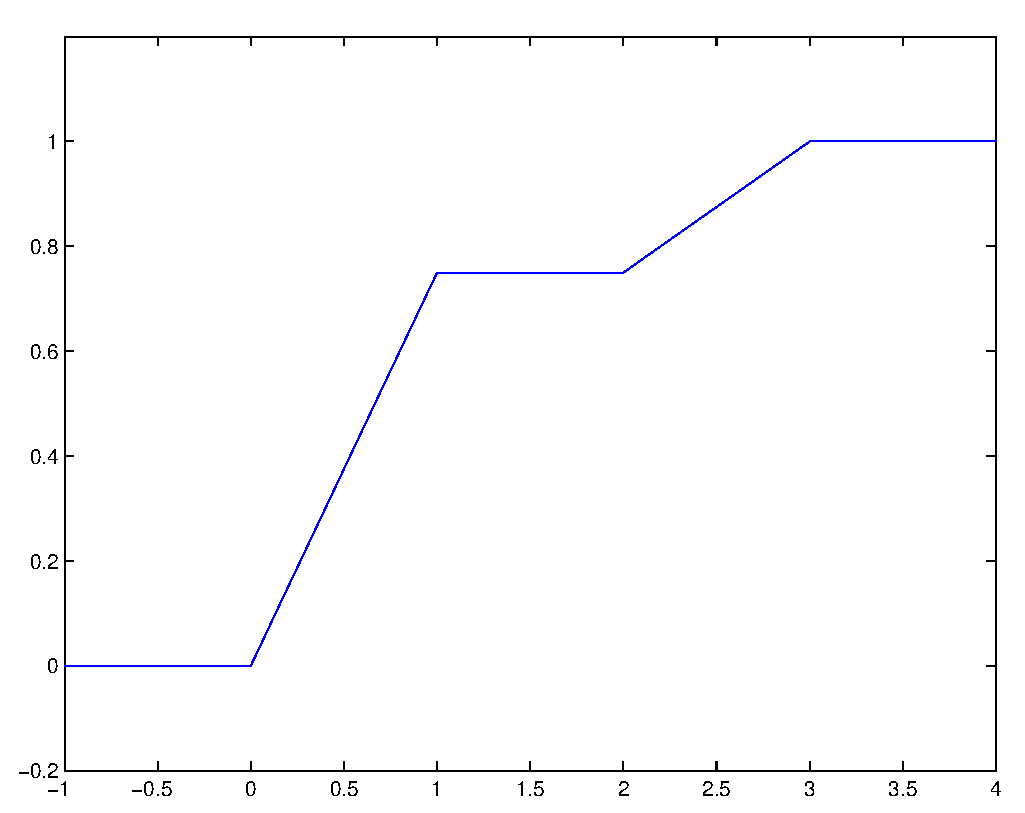
\includegraphics[width=3in, height=1.5in]{ch0501b}
\caption{Distribution function $F(X)$.}
\label{Fig:ch0501b}
\end{figure}

\paragraph*{5.5} The probability density function $f$ of a continuous random variable $X$ is given by: 
\begin{align*}
f(x) = \left\lbrace
\begin{array}{ll}
cx + 3  & \text{for } -3 \leq x \leq -2 \\
 & \\
3- cx  & \text{for }  2 \leq x \leq 3 \\
 & \\
0 & \text{elsewhere.}
\end{array} \right.
\end{align*}

\subparagraph*{a.} Compute $c$. \\
There are two properties for a given probability density function $f$: 
\begin{align*}
& f(x) \geq 0,  \text{ for } -\infty \leq x  \leq \infty \\
& \int_{-\infty}^{\infty} f(x) dx = 1  
\end{align*}
\begin{align*}
\int_{-\infty}^{\infty} f(x) \text{d}x & = \int_{-\infty}^{-3} 0 \text{d}x + \int_{-3}^{-2} (cx + 3) \text{d}x + \int_{2}^3 (3-cx) \text{d}x + \int_{3}^{\infty} 0 \text{d} x \\
& = 0 +  \left[ \frac{cx^2}{2}+3x\right]_{-3}^{-2} + 0 + \left[ 3x - \frac{cx^2}{2}\right]_{2}^3 + 0 \\
& = 0 + \left(\left( \frac{c(-2)^2}{2} + 3(-2) \right) -\left( \frac{c(-3)^2}{2} + 3(-3) \right) \right) + 0 + \left( \left(3(3)-\frac{c3^2}{2} \right) - \left(3(2) - \frac{c2^2}{2} \right) \right) \\
& = 0 + \frac{4c}{2} - 6 - \frac{9c}{2} + 9 + 0 + 9 - \frac{9c}{2} - 6 + \frac{4c}{2} \\
& = 6 -5c = 1 \\
& \Longrightarrow  \\
c & = 1 
\end{align*}

\subparagraph*{b.} Compute the distribution function of $X$.
Given $c=1$, the probability density function is
\begin{align*}
f(x) = \left\lbrace
\begin{array}{ll}
x + 3  & \text{for } -3 \leq x \leq -2 \\
 & \\
3- x  & \text{for }  2 \leq x \leq 3 \\
 & \\
0 & \text{elsewhere.}
\end{array} \right.
\end{align*}

\begin{enumerate}
\item If $a < -3$, then 
\begin{align*}
F(a)   & = \int_{-\infty}^a 0 \text{d} x  \\
& = 0
\end{align*}
\item If $-3 \leq a < -2$, then 
\begin{align*}
F(a) & = \int_{-\infty}^{-3} 0 \text{d} x + \int_{-3}^a (x+3) \text{d} x \\
& = 0 + \left[ \frac{x^2}{2} + 3x\right]_{-3}^{a} \\
& = 0 + \left( \frac{(a)^2}{2} + 3(a)\right) - \left( \frac{(-3)^2}{2} + 3(-3) \right) \\
& = 0 + (\frac{a^2}{2}+3a) - (\frac{9}{2} - 9) \\
& = \frac{a^2+6a+9}{2} \\
& = \frac{(a+3)^2}{2}
\end{align*}
\item If $-2 \leq a < 2$, then
\begin{align*}
F(a) & = \int_{-\infty}^{-3} 0 \text{d} x + \int_{-3}^{-2} (x+3) \text{d} x + \int_{-2}^{a} 0 \text{d} x\\
& = 0 + \left[ \frac{x^2}{2} + 3x\right]_{-3}^{-2} + 0 \\
& = 0 + \left( \frac{(-2)^2}{2} + 3(-2)\right) - \left( \frac{(-3)^2}{2} + 3(-3) \right)  + 0\\
& = 0 + (2-6) - (\frac{9}{2} - 9)  + 0\\
& = \frac{1}{2} 
\end{align*}
\item If $2 \leq a < 3$, then 
\begin{align*}
F(a) & = \int_{-\infty}^{-3} 0 \text{d} x + \int_{-3}^{-2} (x+3) \text{d} x + \int_{-2}^{2} 0 \text{d} x + \int_{2}^a (3-x) \text{d} x\\
& = 0 + \left[ \frac{x^2}{2} + 3x\right]_{-3}^{-2} + 0 + \left[3x - \frac{x^2}{2} \right]_{2}^a \\
& = 0 + \left( \frac{(-2)^2}{2} + 3(-2)\right) - \left( \frac{(-3)^2}{2} + 3(-3) \right) + 0 + \left( \left(3a-\frac{a^2}{2} \right) - \left( 3(2) - \frac{2^2}{2}\right) \right) \\
& = 0 + (2-6) - (\frac{9}{2} - 9) + 0 + \left( 3a - \frac{a^2}{2} -4 \right) \\
& = 0 + \frac{1}{2} + 0 + \frac{6a - a^2 -8}{2} \\
& = \frac{6a - a^2 -7}{2}
\end{align*}
\item If $3 < a$, then
\begin{align*}
F(a) & = \int_{-\infty}^{-3} 0 \text{d} x + \int_{-3}^{-2} (x+3) \text{d} x + \int_{-2}^{2} 0 \text{d} x + \int_{2}^3 (3-x) \text{d} x + \int_{3}^a 0 \text{d} x \\
& = 0 + \left[ \frac{x^2}{2} + 3x\right]_{-3}^{-2} + 0 + \left[3x - \frac{x^2}{2} \right]_{2}^3 + 0 \\
& = 0 + \left( \frac{(-2)^2}{2} + 3(-2)\right) - \left( \frac{(-3)^2}{2} + 3(-3) \right) + 0 + \left( \left(3(3)-\frac{3^2}{2} \right) - \left( 3(2) - \frac{2^2}{2}\right) \right) + 0 \\
& = 0 + (2-6) - (\frac{9}{2} - 9) + 0 + \left( 3(3) - \frac{3^2}{2} -4 \right)  + 0\\
& = 0 + \frac{1}{2} + 0 + \frac{6\times 3 - 3^2 -8}{2} \\
& = 1
\end{align*}
\end{enumerate}
We then plot the distribution function $F(X)$ in Figure~\ref{Fig:ch0505b}, 
\begin{figure}[h!]
\centering
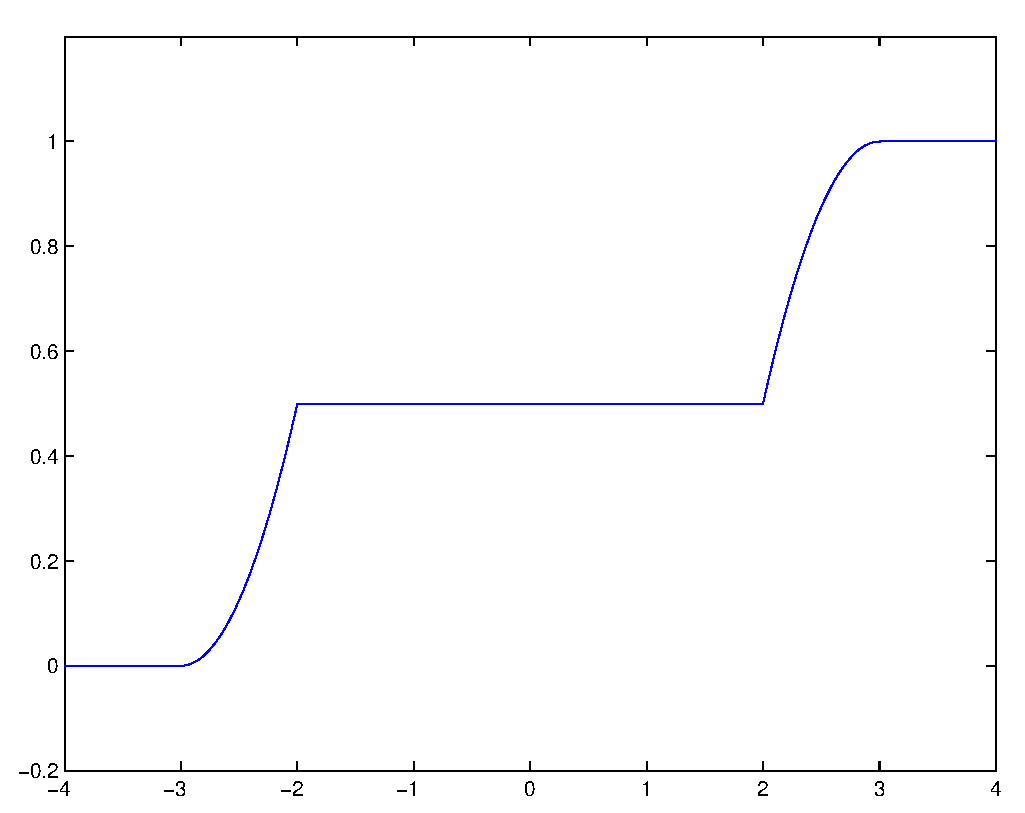
\includegraphics[width=3in, height=1.5in]{ch0505b}
\caption{Distribution function $F(X)$.}
\label{Fig:ch0505b}
\end{figure}
\end{document}
